\documentclass[10pt, conference, compsocconf]{IEEEtran}

%\documentclass{article}

\usepackage{times}
\usepackage{fullpage}
%prevents hyphenating words
%\usepackage[none]{hyphenat} 

%used for pseudocode
\usepackage{algpseudocode}

%used to make charts
\usepackage{pgfplotstable}
\usepackage{pgfplots}

%used for mathematical notation
\usepackage{amsfonts}

%used to switch between amount of columns
%\usepackage{multicol}

%used to control spacing in table captions
\usepackage{subfig}

%used to import images
\usepackage{graphicx}

%used to specify table placement
\usepackage{float}

\renewcommand{\today}{}

\usepackage{aaai_bib}

\title{A Parallel Genetic Algorithm \\For Neural Network Tuning - EXAMPLE VERSION - NOT FOR PUBLIC RELEASE}

\author{Ben Harsha$^1$, Nathan Chadderdon$^2$, Steven Bogaerts$^1$ \\
\\
$^1$Department of Computer Science, DePauw University\\
Greencastle, IN 46135, U.S.A.\\
$^2$Department of Computer Science, Knox College\\
Galesburg, IL 61401, U.S.A.\\
{\tt benjaminharsha\_2015@depauw.edu} \\
{\tt nchadder@knox.edu} \\
{\tt stevenbogaerts@depauw.edu}
}

%define mathematical equations for repeated use
\newcommand{\sigmoid}{$$S(t)=\frac{1}{1+e^{-t}}$$}
\newcommand{\sigmoidprime}{$$S'(t)=S(t) \cdot (1 - S(t))$$}

\begin{document}

\maketitle

\begin{abstract}

One challenge in using artificial neural networks is how to determine appropriate parameters for network structure and learning. Often parameters such as learning rate or number of hidden units are set arbitrarily or with a general ``intuition" as to what would be most effective. The goal of this project is to use a genetic algorithm to tune a population of neural networks to determine the best structure and parameters. This paper considers a genetic algorithm to tune the number of hidden units, learning rate, momentum, and number of examples viewed per weight update. Experiments and results are discussed for two domains with distinct properties, demonstrating the importance of careful tuning of network parameters and structure for best performance.

\end{abstract}

\noindent {\bf Keywords:} Neural network, genetic algorithm, parallelism

\section{Introduction}

Things this paper didn't include in its official version:
\begin{itemize}
\item Itemized lists
\item Enumerated lists
\end{itemize}

Things I wanted to show you how to do here:
\begin{enumerate}
\item Itemized lists
\item Enumerated lists
\end{enumerate}



In the creation of an artificial neural network, low average error on an unseen test set is typically the principle goal. To reach this goal, a network is often trained for many epochs or until a certain average error is achieved on a training set. One risk of such approaches is that they may lead to over-training the network on the training set, hurting its generalizability to the test set. This paper describes a network design technique to reduce average error on a test set by determining ideal structure and parameters. As such, acceptable performance may more likely be reached with reduced need for extra training, and thus reduced risk of over-training. This paper describes a parallel genetic algorithm to tune a population of neural networks, therefore devising an ideal network for a given domain.

\section{Neural Networks}

\begin{figure}
\begin{center}
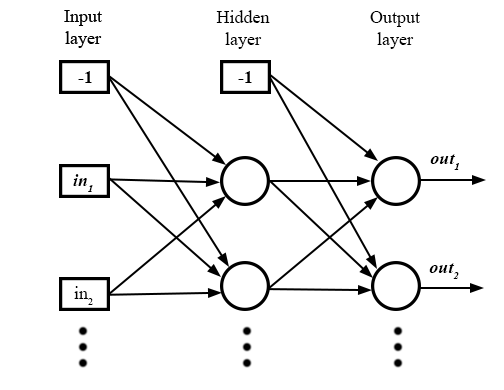
\includegraphics[width=.95\linewidth,height=2.5in]{neuralnetwork.png}
\end{center}
\caption{The structure of a simple neural network}
\label{fig:NN}
\end{figure}

%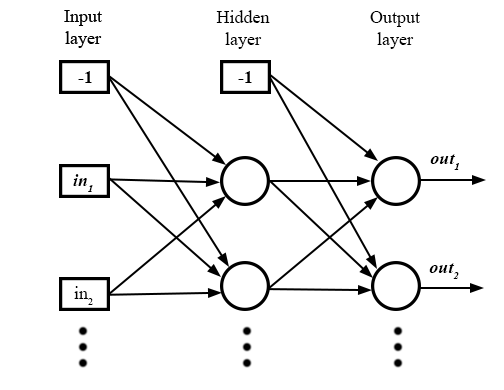
\includegraphics[width = 8cm]{neuralnetwork.png}
%\begin{center}
%\textbf{Figure 1}
%\end{center}

A feed-forward neural network \cite{AImodern} maps a set of inputs into a set of outputs via multiple levels of weighted sums squashed by an activation function. More specifically, inputs are fed into one or more layers of hidden units, which then feed into the output layer. Figure~\ref{fig:NN} shows a feed-forward neural network with a single hidden layer. Each unit's output is computed based on its inputs as follows: 

$$
out_k = S(\sum_{i=1}^n W_{ik}in_{i})
$$
where $n$ is the number of inputs to node $k$, $W_{ik}$ is the weight from input $i$ to node $k$, $in_{i}$ is the input from i, and S is the sigmoid function:
\sigmoid

A network is considered ``trained" when its weights are set such that an appropriate input-output mapping is obtained. For example, a network might take as input the characteristics of a car, and output the value of that car. Back-propagation \cite{AImodern} is one common training process, in which the network considers a training set of input-output examples repeatedly, modifying the weights slightly in response to each example in order to reduce the error on that example. Thus the training process is a form of gradient descent on the error surface with a dimension for each weight in the network. The hope is that in reducing the error on the representative training set, the network's error will also decrease on unseen examples. A measure of network performance can be obtained by finding the average error of the network on a previously-unseen test set of examples, separate from the training set.

In constructing a neural network, a few parameters must be specified: number of epochs for training, number of hidden units, learning rate, momentum, and batch size. All of these variables together determine how the neural network functions, and in the end will have a significant effect on network performance. The remainder of this section describes the meaning of these parameters.

The number of epochs determines how many times a network will train on a training set. A single epoch involves the network examining every example in the training set and adjusting its weights accordingly. In order to actually learn complex functions, this must occur many times -- dozens, hundreds, even thousands, depending on the network and domain.

The number of hidden units determines what kind of functions can be learned by a neural network. Too few means that the target function might not be learnable by the given network. Too many means that the network may take longer to train, may have redundant units that decrease efficiency, or may learn irrelevant details of the inputs that actually harm the generalizability of the network.

The learning rate affects how much the weights are updated during each epoch. If the rate is too high, then the network weights will be adjusted drastically for each example, potentially leading to jumps in the error surface that prevent effective settling at a global minimum. If the rate is too low, then settling may occur quite slowly, requiring more epochs, or even getting stuck in local minima rather than reaching a global minimum.
 
One can imagine a large boulder rolling among steep hills. It will eventually settle at a minimum, but its momentum will determine how much it will move at any given time. The momentum parameter determines how much the ``momentum" of the previous weight change should affect the next. In ideal circumstances, a proper momentum parameter can allow a network to surpass local minima on the way to a global minimum, and can speed up learning in general.

The learning rate and momentum are both used in the weight update rules that follow. For the hidden-output weights:
$$\Delta W_{ji} = \alpha \cdot Err_i \cdot S'(in_i) \cdot x_j + \mu(old\Delta W_{ji})$$
such that
$$in_i = \sum_{j = 1}^n W_{ji}x_j$$
$$Err_i = f_i(\vec{x}) - S(in_i)$$
For input-hidden weights:
$$\Delta W_{kj} = \alpha \cdot x_k \cdot \Delta_j$$
such that
$$\Delta_j = S'(in_j) \cdot \sum_{i} W_{ji} \cdot \Delta_i$$
$$\Delta_i = Err_i \cdot S'(in_i)$$
where $k$ is an input unit index, $j$ is a hidden unit index, $i$ is an output unit index, $f$ is the target function (so $f_i(\vec{x})$ is the activation of output unit $i$ in the known example with inputs $\vec{x}$), $x_k$ and $x_j$ refer to the activation of input and hidden units respectively, $\alpha$ is the learning rate, $\mu$ is the momentum, $W_{xy}$ is the weight from node $x$ to node $y$, $n$ is the number of hidden units, $old\Delta W_{ji}$ is the change made to the weight in the previous update, and $S'$ is the derivative of the sigmoid function:

$$S'(t) = S(t) \cdot (1-S(t))$$

The batch size indicates the number of examples a network examines before updating its edge weights.  With batch sizes greater than one, networks will still compute the new edge weights after each example, but will not update them. It instead computes the change between the new edge weight and the old one. It adds these changes together at each example until it has seen the desired amount, when it finally updates the edge weights. Batch training is used in an effort to be quicker in training a function, although it is not always as accurate.

\section{Genetic Algorithms}

A genetic algorithm \cite{AImodern} is a machine learning algorithm based on the idea of evolution. A population of ``individuals" is rated according to some fitness measure. The most fit individuals are allowed to ``reproduce", passing their genes to their offspring through genetic crossover, thus hopefully improving the fitness of the next generation. Random mutations are also introduced to allow for potentially useful diversity. Thus a genetic algorithm, too, can be thought of as a gradient search: a gradient ascent on a fitness surface, with mutation allowing jumps to other areas of the space to avoid local maxima.

There are many ways in which a genetic algorithm can be applied to neural networks. While it is possible to use a genetic algorithm (instead of back-propagation, for example) to train a network, this is not the approach we take here. Rather, we have applied a genetic algorithm to tune the parameters of a population of neural networks, in order to settle on the ideal network characteristics for a given domain. The parameters under consideration include learning rate, momentum, batch size, and the number of hidden units. The genetic algorithm allows the consideration of a large number of networks, in order to identify broad trends in ideal network parameters. It also enables the development of a final ``ideal" network for a given domain, with performance improved over more arbitrarily-structured networks.

Of course, this approach is computationally expensive, and so we apply parallelism using OpenMP \cite{OpenMP} to improve efficiency. The updating of weights in response to a given example (or batch of examples) is done in parallel, because these updates are independent of each other. In batch learning, multiple examples could also be considered in parallel, with their respective changes accumulated in a shared variable to be applied once at the end of the batch.

While genetic algorithms more commonly store genes as a series of binary values, we chose here to characterize each as a non-negative real number. Thus there are four genes under consideration, corresponding to the network parameters of learning rate, momentum, batch size, and number of hidden units. The genetic algorithm itself also has a number of parameters to determine the operation of the algorithm as applied to a population of neural networks. These parameters are the maximum number of hidden units, maximum learning rate, maximum momentum, maximum batch size, number of individuals, number of generations, removal rate, mutation rate, and testing size. These genetic algorithm parameters are used 

All of the maximum values (hidden units, learning rate, momentum, batch size) are used to create the starting population of networks used in the genetic algorithm, with each network parameter for each network set to various random values between 0 and the maximum value for that parameter. This allows the genetic algorithm freedom to create unique combinations of networks while also limiting the values used in these networks to a reasonable range.

The number of individuals specifies the population size: how many networks are created initially, and how many networks are maintained from one generation to the next. The number of generations is used to determine how many times the algorithm removes poorly-performing networks, and allows more fit networks to reproduce. The removal rate is a decimal between zero and one which gives a percentage of individuals to remove each generation, replaced by the offspring of more fit networks. More specifically, the individuals are sorted based on their average error, and the bottom percentage are removed to be replaced by the children of the top performing individuals. Mutations result in a child not inheriting a trait directly from one of its parents, but instead having a random trait between zero and the maximum value for that trait. This maintains the possibility of useful genetic diversity, while crossover allows the genes the most fit to be passed on. Mutation rate determines how often these mutations occur.

The testing size determines how to split up a data set into training and test sets. Training sets are the examples that are given to the network to have it attempt to learn a function. The test set is then used to determine how well the network was able to learn the function. These sets are created by splitting up the initial data set into two parts based on the value given by testing size. It is given by a decimal between zero and one and determines what percentage of the data will be used for testing, with the remaining percentage being used for training.

\section{Experimental Setup}
\subsection{Data Sets}
The data sets used to train the neural networks were acquired from the UCI Machine Learning Repository \cite{Bache}. Data sets used in experiments include the Car Evaluation Data Set and the Molecular Biology (Splice-junction Gene Sequences) Data Set. These data sets attempt to classify the value of a car given certain characteristics and the type of gene given a genetic sequence.

\subsection{Experiments}
Aside from this more general examining of subjective versus objective, experiments were set up to target specific parameters of both the neural networks and the genetic algorithm in order to find which of these parameters affect the outcome in a meaningful way. One of the goals of these experiments was to see how much better neural networks could do with parameters determined by a genetic algorithm. To determine the difference in the answer between the two, initial experiments were run using only a single neural network. The values used for the parameters of the networks in these experiments were chosen based on what is generally considered reasonable when creating a neural network based on research, past experience, and the size of the data set. For the Cars data set, values of either 5 or 20 were used for the number of hidden units in order to get results from a very low amount and a relatively high one; learning rate and momentum were both kept constant at 0.1 and 0.9 respectively; batch size was varied between 1, 10, and 100 in order to evaluate a range of values. For the Splice data set, values of 10 and 100 were used for the number of hidden units; momentum was again kept constant at 0.9; learning rate varied between 0.1 and 0.3; batch size was kept relatively low, with values of 1 and 10.

An issue that was encountered during experiments involved the program reporting incorrect run times. Eventually, this was determined to be caused by the parallelism. Time was being measured using clock time, so when program branched onto different processors the clock time was altered. This resulted in reported times that were generally three or four times the actual run times measured using a stopwatch. This issue was resolved by using the time function instead of the clock function. Using this method, precision was lost since time only reports in seconds, but the reported times were confirmed to be accurate when compared against a stopwatch.

\section{Results}

\subsection{Cars Data Set Results}

\begin{figure}
\begin{center}
\begin{tikzpicture}
\begin{axis}[width=.95\linewidth,
	xlabel=Number of Epochs,
	ylabel=Average Error, 
	axis lines=left,
	xtick={100, 500, 1000},
	xmin=0, xmax=1100,
	ytick={0.02, 0.04, 0.06, 0.08, 0.1},
	ymin=0,
	scaled y ticks = false,
	y tick label style={/pgf/number format/fixed}]
\addplot [only marks, mark size=1pt] table[y=$avg_err$, x=num_epochs]{carsnumepochs.dat};
\end{axis}
\end{tikzpicture}
\end{center}
\caption{Cars: Effect of the number of epochs on average error.}
\label{fig:CarsNumEpochs}
\end{figure}

Figure \ref{fig:CarsNumEpochs} shows that raising the number of epochs that the networks train on decreases the average error and reduces the variance between average errors calculated by different networks. As shown in the graph above, there is a definite correlation between the number of epochs increasing and the average error decreasing. Along with this, the networks performed more consistently with a higher number of epochs. This is shown by the close proximity of the majority of points at 1000 epochs. It seemed however, that more epochs was not always preferable, as 500 epochs performed better than 1000 on multiple occasions and achieved the lowest average error over all tests.

\begin{table}
\caption{Cars: Amount of results settled below 50\% of maximum batch size.}
\label{tbl:CarsBatchSize}
\centering
\begin{tabular}{c c c}
\hline
Max Batch Size & Total Experiments Run & Below 50\% of Max \\
\hline
50 & 54 & 40 \\
100 & 17 & 17 \\
150 & 8 & 7 \\
\hline
\end{tabular}
\end{table}

When examining batch size, it seems that the genetic algorithm prefers a smaller value. Across all experiments run, the average batch size was 16.4 while the average maximum batch size was 72.2. In addition, among 54 experiments run using a maximum batch size of 50, the batch size settled less than or equal to 25 in 40 of them. This shows that a lower batch size resulted in the neural networks performing better overall. Table~\ref{tbl:CarsBatchSize} summarizes these results. 

\begin{table}
\caption{Amount of results settled below 50\% of maximum hidden units, in the Cars domain.}
\label{tbl:CarsNumHidden}
\centering
\begin{tabular}{c c c}
\hline
Max Hidden Units & Total Experiments Run & Below 50\% of Max \\
\hline
30 & 46 & 34 \\
50 & 8 & 7 \\
100 & 17 & 13 \\
150 & 8 & 7 \\
\hline
\end{tabular}
\end{table}

Similarly, the genetic algorithm tended to settle on a relatively low number of hidden units. Across all experiments, the average value of the maximum hidden units was 60.4 but the average number of hidden units settled on was only 18.2. This average is only 30\% of the average maximum, solidifying that a low number of hidden units was preferable. This clear tendency of settling on low values for number of hidden units is shown by Table \ref{tbl:CarsNumHidden}.

\begin{figure}
\begin{center}
\begin{tikzpicture}
\begin{axis}[width=.95\linewidth,
	xlabel=Momentum,
	ylabel=Average Error,
	axis lines=left,
	xmin=0, xmax=1,
	ytick={0.02, 0.04, 0.06, 0.08, 0.1},
	ymin=0, ymax=0.1,
	scaled y ticks = false,
	y tick label style={/pgf/number format/fixed}]
\addplot[only marks, mark size=1pt] table[y=$avg_err$,x=momentum]{carsmomentum.dat};
\end{axis}
\end{tikzpicture}
\end{center}
\caption{Cars: Effect of momentum on average error.}
\label{fig:CarsMomentum}
\end{figure}

The effect of momentum on the neural networks was nearly indiscernible throughout our experiments. As depicted in Figure \ref{fig:CarsMomentum}, there was no correlation showing that a high or low momentum affected the average error either positively or negatively. Along with this lack of correlation, there did not seem to be any convergence to a high or low momentum value. Throughout tests, it was seemingly random and did not seem to move in any particular direction. Changing the maximum momentum did nothing to change this trend, as results continued to show seemingly unrelated momentums.

\begin{figure}
\begin{center}
\begin{tikzpicture}
\begin{axis}[width=.95\linewidth,
	xlabel=Learning Rate,
	ylabel=Average Error,
	axis lines=left,
	xtick={0.5, 1, 1.5, 2, 2.5},
	xmin=0, xmax=2.5,
	ytick={0.02, 0.04, 0.06, 0.08, 0.1},
	ymin=0, ymax=0.1,
	scaled y ticks = false,
	y tick label style={/pgf/number format/fixed}]
\addplot[only marks, mark size=1pt] table[y=$avg_err$,x=learn_rate]{carslearningrate.dat};
\end{axis}
\end{tikzpicture}
\end{center}
\caption{Cars: Effect of learning rate on average error.}
\label{fig:CarsLearningRate}
\end{figure}

Figure \ref{fig:CarsLearningRate} shows the relationship between the learning rate and the average error. A large portion of experiments were run with a maximum learning rate of 1, so there is a higher concentration of points with a learning rate less than 1. A downward trend was identified after running these tests, suggesting that, in the Cars domain, average error decreases as the learning rate increases. In order to determine if the trend continued with higher learning rates, additional experiments were performed using maximum learning rates up to 5. The results of these experiments continued the downward trend showed previously. Generally, it would seem that increasing the learning rate improves the average error.

Further supporting the idea that higher learning rates are preferred are the learning rates settled on based on the maximum learning rates. Experiments run were broken up into groups based on their maximum learning rate, and the average learning rate for each maximum was computed.

\begin{table}
\caption{Cars: Average learning rate of networks in the final generation, for given maximum possible learning rates.}
\label{tbl:CarsAverageLearningRates}
\centering
\begin{tabular}{c c}
\hline
Maximum Learning Rate & Average Learning Rate \\
\hline
5 & 1.7267 \\
2 & 1.4079 \\
1.5 & 1.2643 \\
1 & 0.6367 \\
0.75 & 0.4205 \\
0.5 & 0.3656 \\
0.3 & 0.26 \\
0.1 & 0.0818 \\
\hline
\end{tabular}
\end{table}

For each maximum learning rate Table \ref{tbl:CarsAverageLearningRates} except 5, the average learning rate is in the upper 50\% of the possible range. This confirms that the genetic algorithm tends to settle on higher learning rates relative to the maximum learning rate, but also shows that there is a threshold in which increasing the learning rate is no longer effective in improving the average error.

\begin{table}
\caption{Cars: Average error over all networks with given number of individuals.}
\label{tbl:CarsIndividuals}
\centering
\begin{tabular}{c c}
\hline
Number of Individuals & Average Error \\
\hline
10 & 0.0421816786 \\
20 & 0.0347347333 \\
30 & 0.0283559333 \\
\hline
\end{tabular}
\end{table}

\begin{table}
\caption{Cars: Average error over all networks with given number of generations.}
\label{tbl:CarsGenerations}
\centering
\begin{tabular}{c c}
\hline
Number of Generations & Average Error \\
\hline
10 & 0.0417958082 \\
20 & 0.0356072 \\
30 & 0.031888 \\
\hline
\end{tabular}
\end{table}

Increasing the number of individuals and generations in the genetic algorithm had the effect of making the networks perform more consistently, but not necessarily better. The majority of tests were run using ten individuals running for ten generations. These amounts were varied in independent experiments in order to determine whether they made any difference on the networks' ability to learn the function. The result of these experiments showed that increasing both of these values had a noticeably positive effect on the networks. While the networks with larger generations and individuals did not get the best error over all tests, they proved to be the most consistent out of all groups tested. Especially those with thirty individuals running ten generations and those with ten individuals running thirty generations were near the top in terms of average error regardless of the number of epochs used to train them.

\subsection{Splice Data Set Results}

\begin{figure}
\begin{center}
\begin{tikzpicture}
\begin{axis}[width=.95\linewidth,
	xlabel=Number of Epochs,
	ylabel=Average Error, 
	axis lines=left,
	xtick={10, 50, 100},
	xmin=0, xmax=110,
	ytick={0.02, 0.04, 0.06, 0.08, 0.1},
	ymin=0, ymax = 0.06,
	scaled y ticks = false,
	y tick label style={/pgf/number format/fixed}]
\addplot [only marks, mark size=1pt] table[y=$avg_err$, x=num_epochs]{splicenumepochs.dat};
\end{axis}
\end{tikzpicture}
\end{center}
\caption{Splice: Effect of the number of epochs on average error.}
\label{fig:SpliceNumEpochs}
\end{figure}

Similar tests were performed on the Splice data set in order to consider both general trends and trends specific to each data set. As shown in Figure \ref{fig:SpliceNumEpochs}, the effect that varying the number of epochs had on the average error was extremely similar to the Cars domain. Average error slightly decreased from 10 epochs to 50 epochs, but the effect was much less apparent from 50 epochs to 100 epochs. Again, there was even some performance lost when comparing networks with fifty epochs to those with 100.

\begin{table}
\caption{Splice: Amount of results settled below 50\% of maximum batch size.}
\label{tbl:SpliceBatchSize}
\centering
\begin{tabular}{c c c}
\hline
Max Hidden Units & Total Experiments Run & Below 50\% of Max \\
\hline
20 & 29 & 19 \\
100 & 23 & 23 \\
\hline
\end{tabular}
\end{table}

Also similar to the Cars domain was the genetic algorithm's preference to settle on low batch sizes. Across all experiments run, the average maximum batch size given to the genetic algorithm was 50.1, while the average batch size settled on was just 11.3. Table \ref{tbl:SpliceBatchSize} shows this convergence to lower values. Once again, this conveys that the neural networks are able to perform consistently better when given a lower batch size.

\begin{figure}
\begin{center}
\begin{tikzpicture}
\begin{axis}[width=.95\linewidth,
	xlabel=Number of Hidden Units,
	ylabel=Average Error,
	axis lines=left,
	xmin=0, xmax=100,
	ytick={0.02, 0.04, 0.06, 0.08, 0.1},
	ymin=0, ymax=0.06,
	scaled y ticks = false,
	y tick label style={/pgf/number format/fixed}]
\addplot[only marks, mark size=1pt] table[y=$avg_err$,x=num_hidden]{splicenumhidden.dat};
\end{axis}
\end{tikzpicture}
\end{center}
\caption{Splice: Effect of number of hidden units on average error.}
\label{fig:SpliceNumHidden}
\end{figure}

Examining the behavior of the number of hidden units showed similarities to those shown by the Cars data set. In general, the algorithm preferred to settle on values that were relatively low given their maximum range. Figure \ref{fig:SpliceNumHidden} shows the wider range chosen by the ideal networks in the Splice data set.

\begin{figure}
\begin{center}
\begin{tikzpicture}
\begin{axis}[width=.95\linewidth,
	xlabel=Momentum,
	ylabel=Average Error,
	axis lines=left,
	xmin=0, xmax=1,
	ytick={0.02, 0.04, 0.06, 0.08, 0.1},
	ymin=0, ymax=0.06,
	scaled y ticks = false,
	y tick label style={/pgf/number format/fixed}]
\addplot[only marks, mark size=1pt] table[y=$avg_err$,x=momentum]{splicemomentum.dat};
\end{axis}
\end{tikzpicture}
\end{center}
\caption{Splice: Effect of momentum on average error.}
\label{fig:SpliceMomentum}
\end{figure}

The effects of momentum were still not discernible from the results gathered using the Splice data set. As shown in Figure \ref{fig:SpliceMomentum}, momentum's influence was again seemingly random. No trends were found that gave any evidence that momentum affected the average error in either a positive or negative way.

\begin{figure}
\begin{center}
\begin{tikzpicture}
\begin{axis}[width=.95\linewidth,
	xlabel=Learning Rate,
	ylabel=Average Error,
	axis lines=left,
	xtick={0.5, 1, 1.5, 2, 2.5},
	xmin=0, xmax=2.5,
	ytick={0.02, 0.04, 0.06, 0.08, 0.1},
	ymin=0, ymax=0.06,
	scaled y ticks = false,
	y tick label style={/pgf/number format/fixed}]
\addplot[only marks, mark size=1pt] table[y=$avg_err$,x=learn_rate]{splicelearningrate.dat};
\end{axis}
\end{tikzpicture}
\end{center}
\caption{Splice: Effect of learning rate on average error.}
\label{fig:SpliceLearningRate}
\end{figure}

The trend of the algorithm preferring a higher learning rate did not continue over the Splice data set. Even when given freedom to choose higher values, the most effective networks usually used learning rates that were much lower than those used by the Cars data set. Figure \ref{fig:SpliceLearningRate} shows this convergence toward lower learning rates while also showing that the higher learning rates do not typically out-perform the lower ones.

\begin{table}
\caption{Splice: Average learning rate of networks in the final generation, for given maximum possible learning rates.}
\label{tbl:SpliceAverageLearningRates}
\centering
\begin{tabular}{c c}
\hline
Maximum Learning Rate & Average Learning Rate \\
\hline
5 & 0.9623 \\
3 & 0.758 \\
1 & 0.472 \\
0.5 & 0.3141 \\
0.3 & 0.1955 \\
\hline
\end{tabular}
\end{table}

In Table \ref{tbl:SpliceAverageLearningRates}, it is significant that the groups with higher maximum learning rates have such relatively low average learning rates because this shows that even when given the option to have higher learning rates, the genetic algorithm does not choose the higher values. On the other end, however, the groups with lower maximum learning rates do tend to settle on values that are relatively high for the range.

\begin{table}
\caption{Splice: Average error over all networks with given number of individuals.}
\label{tbl:SpliceIndividuals}
\centering
\begin{tabular}{c c}
\hline
Number of Individuals & Average Error \\
\hline
10 & 0.0362218463 \\
20 & 0.0302012667 \\
30 & 0.0291261667 \\
\hline
\end{tabular}
\end{table}

\begin{table}
\caption{Splice: Average error over all networks with given number of generations.}
\label{tbl:SpliceGenerations}
\centering
\begin{tabular}{c c}
\hline
Number of Generations & Average Error \\
\hline
10 & 0.0354922167 \\
20 & 0.0370337333 \\
30 & 0.0354270333 \\
\hline
\end{tabular}
\end{table}

Increasing the number of individuals and generations had a very similar effect to what was examined with the Cars data set, as seen in Tables \ref{tbl:SpliceIndividuals} and \ref{tbl:SpliceGenerations}. As those two values increased, the networks were able to learn the functions at a more consistent level. Once again, the networks run with higher amounts of generations and individuals did not achieve the best overall average errors, but they consistently performed at a high level.

\section{Analysis}

In the results section above, it was determined that a higher number of epochs results in a generally lower average error. From the beginning of the process, this was expected. Results of experiments were able to confirm expectations by showing a clear improvement in average error from 100 to 500 epochs in the Cars data set, and from 10 to 50 in the Splice data set. Neural networks need a large number of epochs to learn functions, and it is intuitive that more epochs would cause the network to learn a function more effectively. What was not expected, however, was that simply adding more epochs does not always improve the performance of the neural networks. In Figure \ref{fig:CarsNumEpochs}, it is apparent that networks with 500 epochs routinely performed just as well or better than networks with 1000 epochs, and a similar trend was shown in Figure \ref{fig:SpliceNumEpochs}. It is possible that the higher number of epochs is leading to over-training. This is one drawback of simply training for a certain number of epochs, instead of considering an error-based stopping criterion.

It was also revealed that the genetic algorithm tended to settle on a smaller batch size in both data sets being tested. The purpose of batch training is to make cumulative, less frequent changes to the network, to prevent frequent changes in response to individual examples. On the other hand, making corrections for one example at a time may allow better performance and more refined corrections on the next. Therefore there is a balance to be struck. The genetic algorithm suggests that smaller batch sizes are preferred, at least in the Cars and Splice domains, suggesting that overall each example provides useful information towards the target function and is best applied quickly to the weights.

The results involving hidden units are a bit harder to interpret. In the Cars domain there is a clear negative correlation between the number of hidden nodes and the error, while in the Splice domain the number of hidden units doesn't seem to have a significant impact on the error. There is clearly some difference between domains that makes some more sensitive to the number of hidden units than others, but without further testing it is difficult to say just what that difference might be.

As noted above, momentum did not have a significant effect on the experiments being run, with no correlation between momentum and average error, and no convergence to a specific momentum value across all experiments. The purpose of momentum is to avoid settling on a local minimum. It could be that momentum was not affecting our results because the local minimum was often also a global, or it could be that momentum simply does not have a drastic effect on the datasets being used for these experiments.

It was expected to see that increasing the number of individuals and generations led to more consistently solid performance from the neural networks based on the model presented by the genetic algorithm. Using more individuals gives the algorithm a broader range of data to work with, so it has more options to explore when attempting to evolve the optimal network. It follows then that the resulting networks should be more effective than those coming from a genetic algorithm with fewer individuals. Similarly, using a higher number of generations allows the algorithm more time to evolve and tune the genes. This also results in networks that will have more consistent traits and answers.

When examining the effect of learning rate on the neural networks, it was very surprising that for the Cars domain, a higher learning rate resulted in lower average errors, although there did seem to be a point where a higher learning rate stopped being effective. Only one genetic algorithm finished with a learning rate over 2, even though maximum values of 3 and 5 were used for multiple experiments. Assumptions going into experiments were that a learning rate lower than 0.5 was ideal. As shown in Figure \ref{fig:CarsLearningRate}, however, this is not always the case. Networks with higher learning rates were able to consistently perform on par or better than networks with learning rates around the previously considered ideal range. This is most likely caused by the relatively small amount of epochs used in the experiments. Since the data sets were so large, it was not feasible to test them for hundreds of thousands of epochs. It was necessary to keep the number of epochs low in order to perform experiments in an efficient manner. Because of these low numbers of epochs, it makes sense that a higher learning rate would benefit the network. It has less time to learn the function, so a higher learning rate speeds up the process by making larger changes each time the network's weights are updated.

\section{Related Work}

The parallelization of neural networks has been the focus of much research. For example, \cite{Kim} describes a parallel training algorithm similar to the one in this paper, in which the weight updates are computed in parallel by breaking the updates into steps and running them through a pipeline.

Work has also been done in the application of parallelism to genetic algorithms of neural networks. \cite{Gruau} describes a genetic algorithm used to find an optimal neural network to simulate a Turing machine. Parallelism was applied by separating the genetic algorithm population into separate ``islands", with the goal of increasing overall genetic diversity. This is in contrast to the work of this paper, in which the members of the next generation are created in parallel, but all individuals were in the same group together.

Another example of a genetic algorithm applied to neural networks can be found in \cite{Soares}. That work focuses on the creation of neural network ensembles -- groups of neural networks that work together to come to a decision. As a part of the ensemble generation, the individual neural networks were optimized using parameters and genes similar to those used in this project. Most similar to the work performed in this paper were the initialization of weights in the network and the use of the number of hidden units as a gene in the genetic algorithm phase.

\section{Future Work}

The work described in this paper leads to many questions for further research. With the limited time available for this research, it was only possible to explore two domains. An expansion of the data sets investigated may uncover more patterns that could guide network design more deeply. It would be very interesting to attempt to develop some guidelines for network design given the domain characteristics; experimentation on many more domains may make that kind of analysis possible. One specific trait that merits further investigation is how much the subjectivity/objectivity of the domain affects the performance of a network. For example, it was noted that in the two domains tested that the Cars domain, which is more subjective, ends up with a higher learning rate than the Splice domain, which is more objective.

More work would also be useful in identifying properties of the domain that affect what parameters like the learning rate should be. The learning rate chosen by the genetic algorithm varied in the two domains, with the Cars domain favoring higher learning rates and the Splice data set favoring more traditional lower learning rates. More work may be able to determine what about the Cars domain makes a higher learning rate favorable, allowing others to know what learning rate will give them the best results without having to simply try them all.

The two domains also differed in their results regarding number of hidden units, while neither seemed influenced by the momentum parameter. We would like to explore possible explanations for this in more detail.

\section{Conclusion}
This paper describes results of experiments using a parallel genetic algorithm to tune neural network design. In particular, the algorithm considered the number of hidden units, learning rate, momentum, number of training epochs, and batch size. The domains behaved similarly in some of these parameters, but quite differently in others. Specifically, the Cars domain preferred a higher learning rate and a lower number of hidden units. Both domains preferred a moderate amount of epochs (around 500) and a smaller batch size, and neither seemed particularly influenced by the momentum parameter. Some potential explanations are offered, and these results lead to additional questions to be considered, particularly in applying this work to a greater number of domains.

\section{Acknowledgement}
This work was supported by NSF grant number CNS-1156893.

\bibliographystyle{aaai}
\bibliography{parallelNNGA}

\end{document}
